%!TEX root = ../surface_reconstruction.tex
\phantomsection
\section*{Аннотация}
\addcontentsline{toc}{section}{Аннотация}
Работа посвящена задаче реконструкции поверхности - классической задаче
обработки цифрового представления отсканированной физической формы. 
Существует большое количество методов, восстанавливающих поверхность 
по набору дискретных точек. В данной работе рассматривается метод движущихся 
наименьших квадратов, выделяющийся тем, что вычисляет точечное представление 
результирующей поверхности и устойчивостью к зашумлённости входных данных. 
Предложен параллельный вариант алгоритма, предназначенный для распределённой вычислительной 
системы. Вычислительные эксперименты, проведённые на высокопроизводительном кластере Polus, показали
хорошую масштабируемость предложенной реализации метода движущихся 
наименьших квадратов.
\clearpage

\section*{Введение} 
\addcontentsline{toc}{section}{Введение}
В настоящее время активно развивается область геометрического моделирования и построение 3D моделей по облакам точек, полученным с лазерных сенсоров. Одной из базовых задач геометрического моделирования является реконструкция поверхности по облаку точек. У методов реконструкции поверхностей широкий спектр применения: 
\begin{itemize}
    \item реконструкция поверхности применяется при распознавании лиц;
    \item реконструкция поверхности применяется при построении трехмерных моделей объектов с использованием таких сенсоров как лидар и камера глубины;
    \item в робототехнике в задачах локализации и построение трехмерных карт на основе облаков точек с сенсоров реконструкция является важным этапом задачи;
    \item реконструкция поверхности применяется в медицине;
    \item реконструкция поверхности применяется в машинном зрение;
\end{itemize}

Очень интересным и перспективным является применение методов реконструкции поверхности в 3D картографии. Для построения точной карты требуется длительный и дорогой труд разметчиков. Одним из направлений в автоматизации этого процесса является следующее решение. Записывается баг файл с данными с лидара и камеры (скан с лидара и снимок с камеры синхронизирован по времени) при движении автомобиля по улице.  К снимкам с камеры применяется сегментирующая нейронная сеть (см. рис. \ref{fig:-2}), к сканам с лидара применяется алгоритм реконструкции(повышается дискретизация, заполняются пропуски, удаляется шум, выбросы), затем облако точек проецируется на маску, полученную решением нейронной сети(это возможно благодаря внутренней калибровки камеры(матрицы проекции) и внешней калибровки(перехода от системы координат лидара в систему координат камеры (вектор сдвига и поворотов))). Используя взаимно-однозначное соответствие между данными с лидара и камеры облако точек также сегментируется(см. рис. \ref{fig:-2}).
\begin{figure}[h]
    \centering
    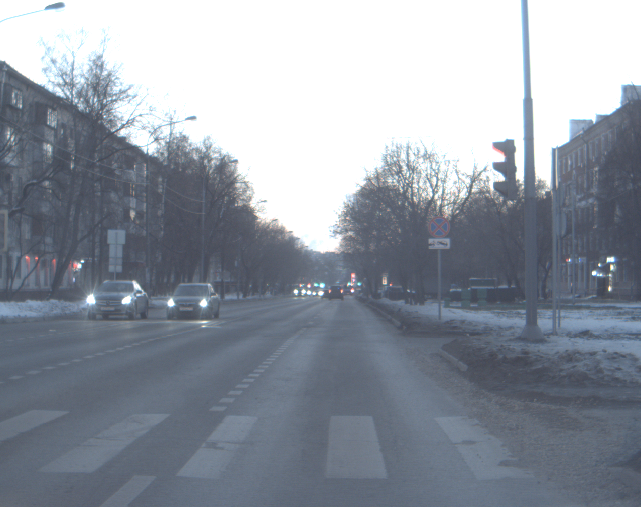
\includegraphics[width=0.32\textwidth, height=5cm]{images/image.png}
    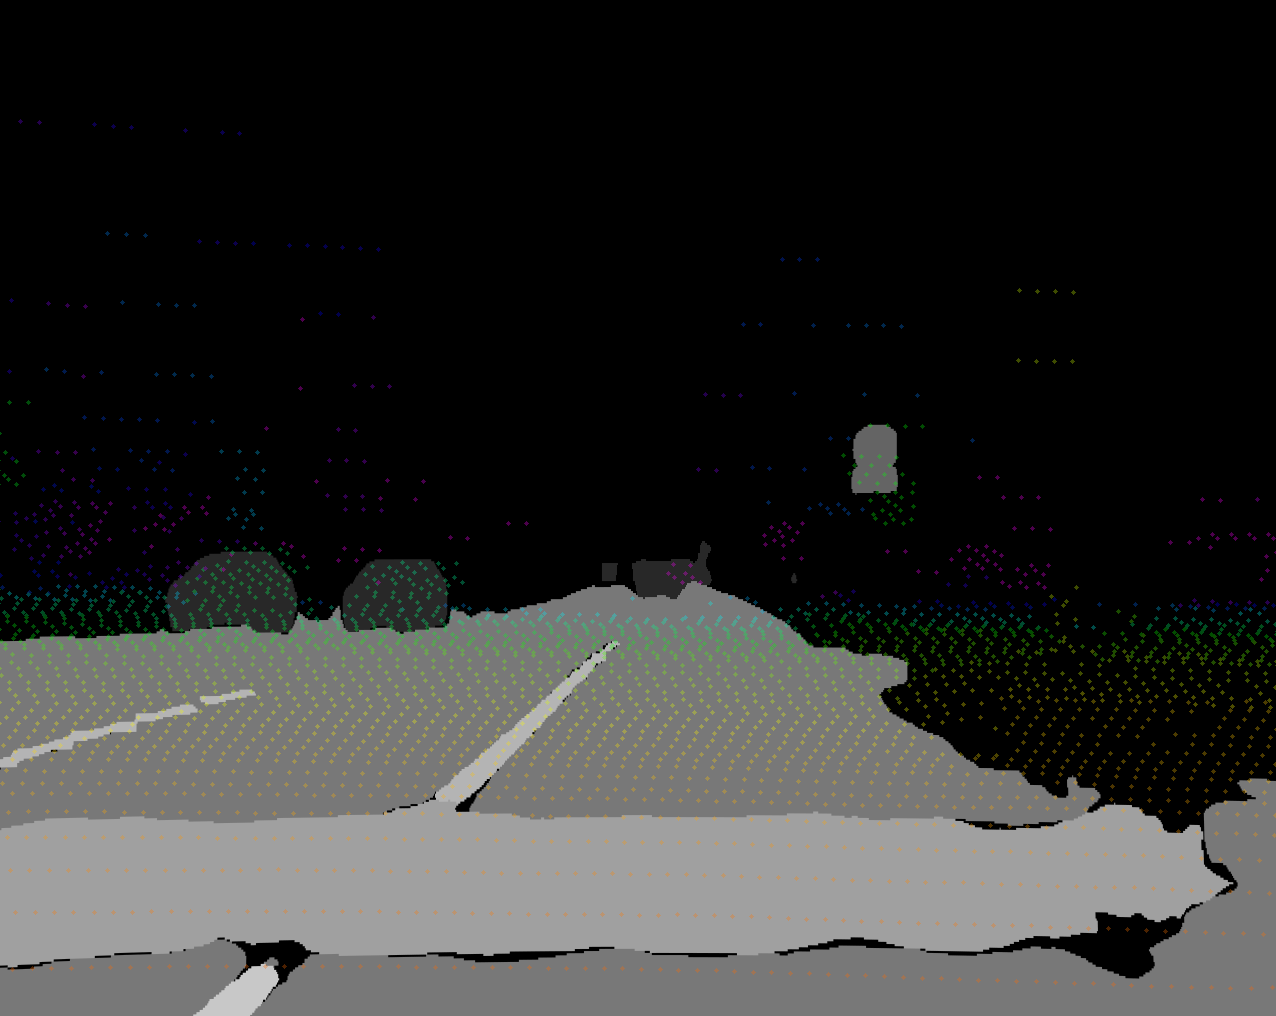
\includegraphics[width=0.32\textwidth, height=5cm]{images/mask.png}
    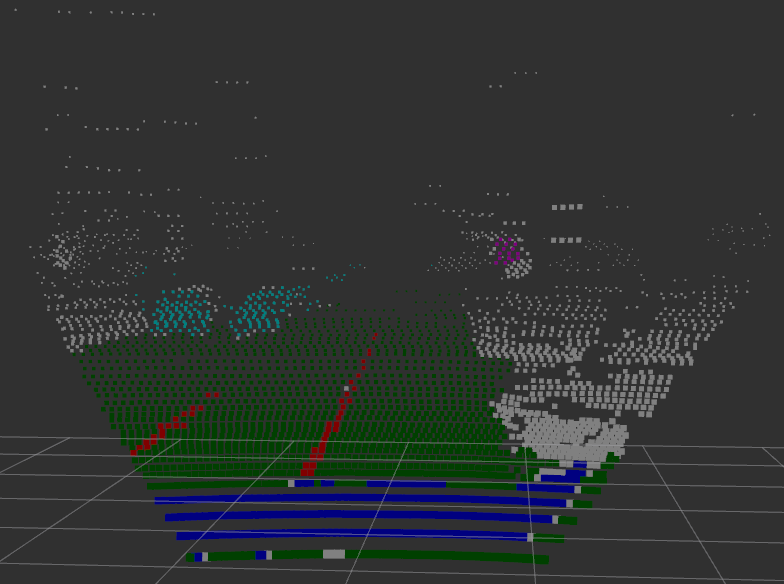
\includegraphics[width=0.32\textwidth, height=5cm]{images/painted_cloud.png}
    \caption{Сегментирование облака точек с использованием маски сегментированного изображения и взаимно-однозначного соответствия между данными с лидара и камеры.}
    \label{fig:-2}
\end{figure}

\newpage

Сканы с лидара склеиваются в один непрерывный скан (см. рис. \ref{fig:-1})

\begin{figure}[h]
    \centering
    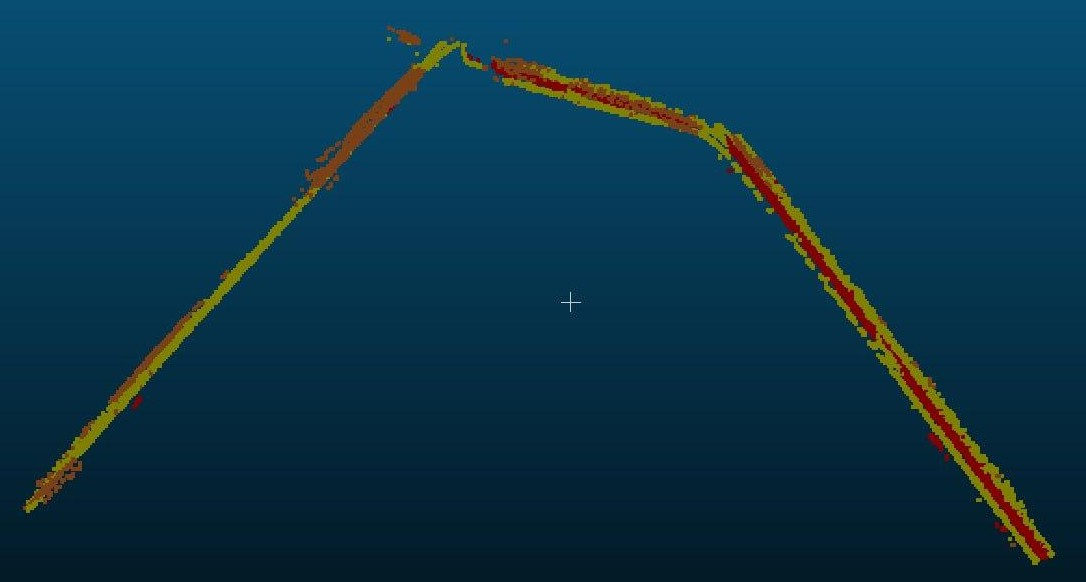
\includegraphics[width=0.8\textwidth, height=5cm]{images/glued.jpg}
    \caption{Склеенные сегментированные сканы с лидара.}
    \label{fig:-1}
\end{figure}

К зданиям с улицы также применяются алгоритмы реконструкции для задания их полигональной сеткой (см. рис. \ref{fig:street}).

\begin{figure}[h]
    \centering
    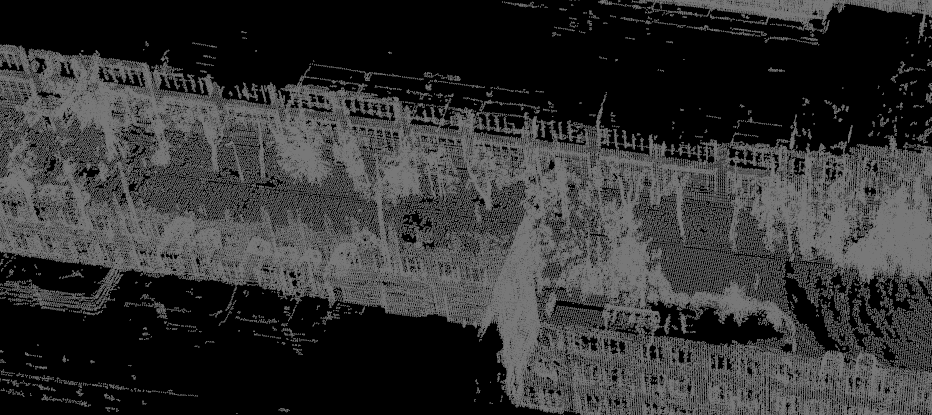
\includegraphics[width=0.8\textwidth, height=5cm]{images/street.png}
    \caption{Склеенные сканы домов улицы.}
    \label{fig:street}
\end{figure}

В связи с резким повышением доступности лидарных сенсоров, на сегодняшний день их можно увидеть на некоторых моделях популярных телефонов(iphone 12 pro и др.). Это поспособствовало появлению многочисленных стартапов связанных с изготовлением ортопедической обуви по индивидуальному слепку ноги полученному с помощью сканирования и последующей реконструкции поверхности стопы. При изготовлении профессиональной спортивной экипировки (такой как коньки, шлемы) используется трёхмерное сканирование соответствующих частей тела для получения слепка.


В первом разделе работы проводится обзор теории, рассматриваются методы реконструкции поверхности представляющие поверхность сеткой, а также набором точек высокой дискретизации. Рассмотрены алгоритмы триангуляции Делоне, поверхности алгебраических точек, метод движущихся наименьших квадратов.

Во втором разделе описывается особенности параллельной реализации алгоритма MLS. Алгоритм обладает большим ресурсом параллелизма из-за своей локальности вычислений, а также отсутствием проблемы объединения кусков поверхности ввиду точечного представления поверхности(в отличие от сеточного). В разделе представлена схема параллельного алгоритма, а также графы информационной зависимости распараллеленных циклов. При вычислении полинома, задающего точки поверхности MLS, для точки в пространстве(точка запроса), нужно выполнить поиск по всему облаку точек, чтобы найти элементы, входящие в сферу радиуса \textbf{r} (параметр метода) и центром в точке запроса. Это стандартная задача пространственного индексирования, которую можно ускорить с помощью различных структур данных. Наиболее часто, для этой задачи используется k-d дерево ~\cite{Russell}, так как его легко построить и выполнять по нему запросы. Алгоритм пользуется тем, что входные данные, например скан с лидара, при разбиении, представляют непрерывные части поверхности. Таким образом, при построении k-d деревьев, в них оказываются точки с непрерывных частей поверхностей, что исключает необходимость в использование данных k-d деревьев с соседних процессов. В случае, когда порядок точек в облаке хаотичен, можно воспользоваться одним из методов сортировки точек, например, переупорядочить в порядке Мортона ~\cite{MORTON}. В разделе, также представлен порядок вычислительной сложности различных этапов алгоритма. Нелинейная вычислительная сложность этапа построения k-d дерева, приводит к тому, что увеличение количества деревьев связанное с увеличением количества процессов, ведет к нелинейному уменьшению количества операций выполняемых на процессе, что благотворно сказывается на эффективности алгоритма.

Третий раздел содержит результаты работы параллельного алгоритма на суперкомпьютере, их анализ, выводы и рекомендации.




Проблема определения поверхности по набору точек активно изучается многие годы. Несмотря на распространение методов реконструкции поверхности, многие аспекты проблемы остаются открытыми. Большинство алгоритмов восстановления поверхности представляют поверхность сеткой. Но существуют также алгоритмы, которые представляют поверхность набором точек с высокой дискретизацией.

Одними из основных трудностей в процессе реконструкции являются сложность формы и шум. В центре внимания работы алгоритм восстановления поверхности в основе которого метод наименьших квадратов, в связи с чем алгоритм получил название метод движущихся наименьших квадратов(Moving Least Squares). Алгоритм называется движущимся поскольку итеративно двигается по набору точек. Данный алгоритм имеет различные вариации. Наиболее используемым вариантом является проекционный оператор MLS. Проекционный оператор MLS ~\cite{LEVIN} зарекомендовал себя как мощный метод реконструкции поверхности. 
Метод MLS позволяет достичь простого и эффективного представления поверхности набором точек. В настоящее время поверхности MLS широко применяются при обработке и рендеринге моделей с точечной выборкой и все чаще используются в качестве стандартного определения поверхностей набором точек.  Вычисление точек на поверхности является локальным, что приводит к нестандартной методике, которая может обрабатывать любой набор точек. Помимо реконструкции поверхности функцией сглаживания, у метода движущихся наименьших квадратов есть много других преимуществ, таких как внутренняя способность обрабатывать входные данные с шумом, простота вычисления дифференциальных геометрических свойств поверхности (например, нормали, кривизны).

В дифференциальной геометрии гладкая поверхность характеризуется существованием гладких локальных отображений в любой точке.  MLS предоставляет такое отображение на локальной области определения, локальной системы координат. И хотя формально, можно задать поверхность MLS неявными функциями, на практике эти функции аппроксимируются набором точек с этих функций, с дискретизацией порядка разрешения изображения. Это связано с большим количеством полиномов, сложностью пересчета их как неявных функций к общей системе координат и задания области их определения, и других неоднозначных проблем. В работе ~\cite{LEVIN} показано, что ошибка такой аппроксимации ограничена и зависит от расстояния между точками. Таким образом, можно обеспечить наперед заданную точность приближения поверхности. Существует много различных вариантов алгоритма MLS, но в основном они отличаются выбором локальной области определения.

Улучшение качества поверхности или улучшение визуального качества геометрической поверхности субъективно. Утверждение, что один метод обеспечивает лучшее качество поверхности, может варьироваться от человека к человеку. По этой причине необходимо установить численные меры для сравнения влияния алгоритмов восстановления поверхности на качество поверхности.
В геометрическом моделировании для описания уровня искажения поверхности используется величина, называемая среднее геометрическое отклонение(average geometric deviation). В работе также считается среднеквадратичное отклонение(standard deviation).



% \begin{figure}
%     \centering
%     \subfigure[]{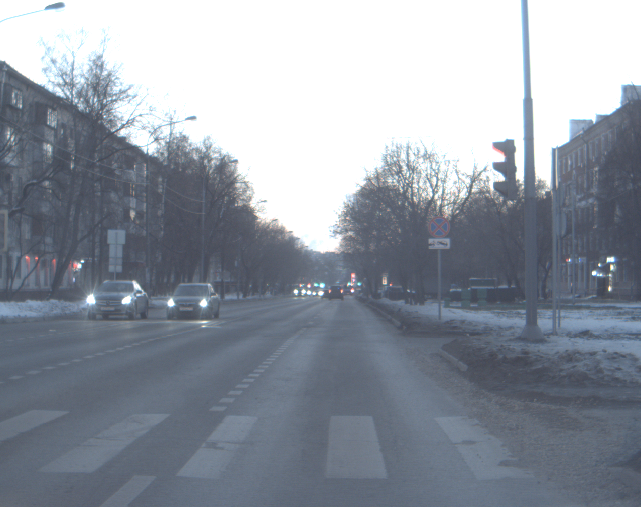
\includegraphics[width=0.24\textwidth]{images/image.png}} 
%     \subfigure[]{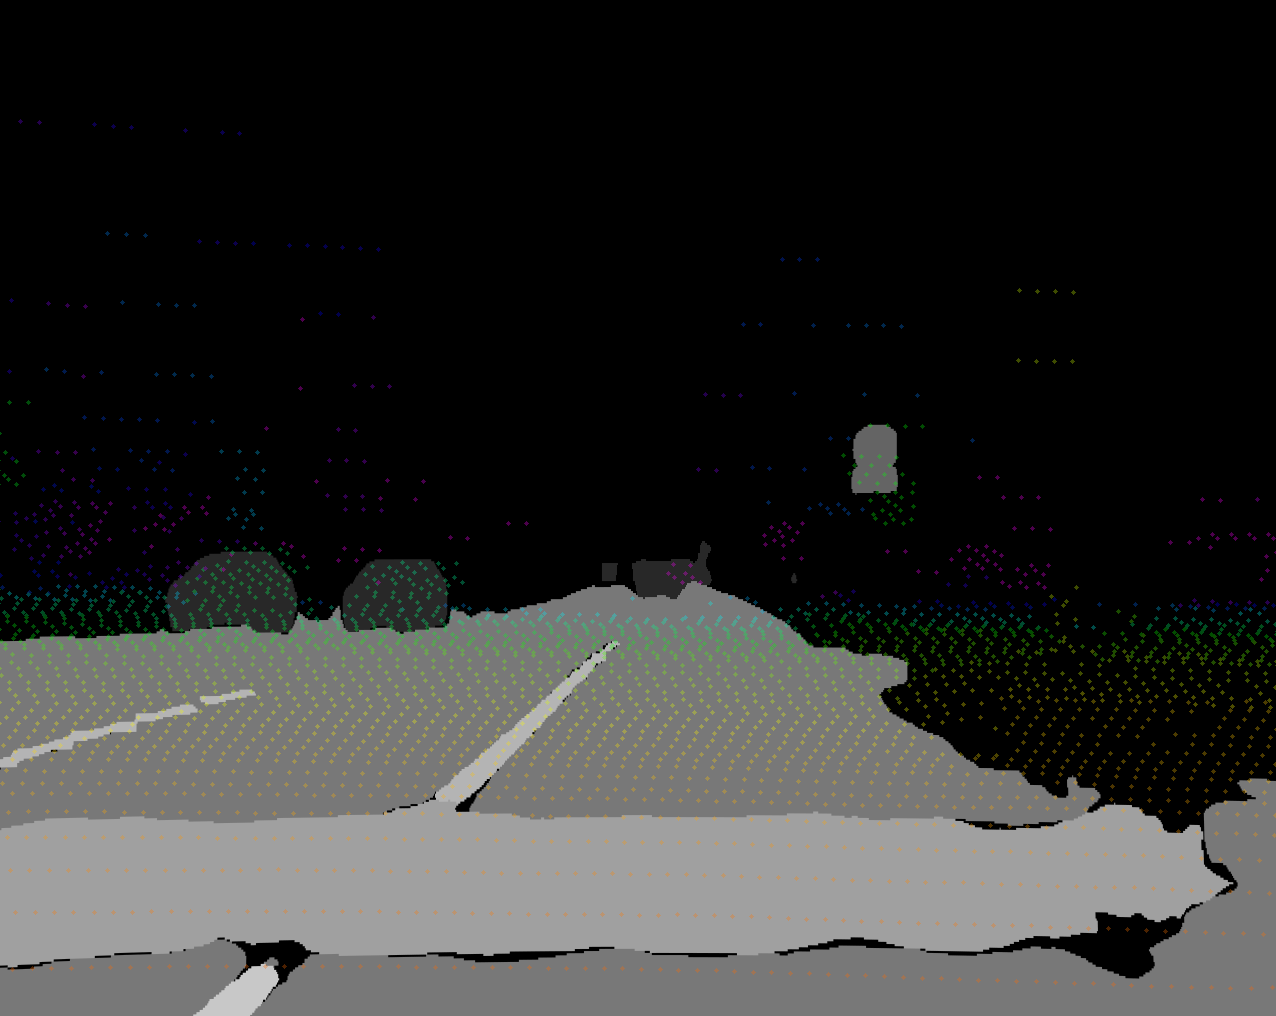
\includegraphics[width=0.24\textwidth]{images/mask.png}} 
%     \subfigure[]{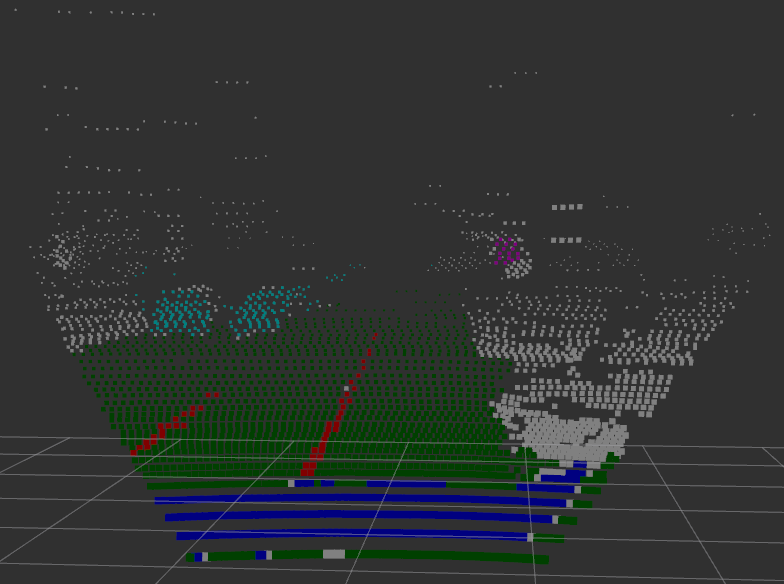
\includegraphics[width=0.24\textwidth]{images/painted_cloud.png}}
%     \caption{(a) blah (b) blah (c) blah}
%     \label{fig:foobar}
% \end{figure}



\textbf{Практическая значимость} работы состоит в возможности использования ее результатов для широкого круга применений, требующих восстановления поверхности по облаку точек. Данная работа может помочь разработчику выбрать оптимальный метод реконструкции поверхности.

\section*{Цель работы и задачи}
\addcontentsline{toc}{section}{Цель работы и задачи}
\textbf{Целью} настоящей работы является разработка параллельного метода восстановления поверхности, основанного на методе наименьших квадратов, на суперкомпьютере с распределенной памятью, позволяющего добиться оптимальных результатов как в масштабируемости, так и в качестве восстановления поверхности.

\textbf{Задачами} работы являются: 
\begin{itemize}
    \item Разработка параллельного алгоритма восстановления поверхности методом движущихся наименьших квадратов на распределенной памяти;
    \item Написание гибридной программы восстановления поверхности на распределенной памяти с использованием библиотек MPI и openMP;
    \item Тестирование разработанного алгоритма и оценка его эффективности, ускорения, масштабируемости, а также качества восстановленной поверхности по среднеквадратичному отклонению (standard deviation) и среднему геометрическому отклонению(average geometric deviation) от эталонной поверхности;
\end{itemize}
